\section{Ejercicio 3}
\subsection{El Problema}
Se tiene una matriz $M$ de tamaño $CxA$. Se tiene una función \texttt{sueldo} que dados un cargo $c_1$ y una antigüedad $a_1$ devuelve un número que se calcula con la siguiente fórmula.

\texttt{sueldo}($c_1$,$a_1$) = $\sum_{i=1}^{c} \sum_{j=1}^{a} M_{i,j}$

Dadas antigüedades $a_1$ y $a_2$ y cargos $c_1$ y $c_2$, se quiere poder calcular la parte de \texttt{sueldo}($a_2$,$c_2$) que jamás podrá ser alcanzada teniendo antigüedad $a_1$ o cargo $c_1$. Se llamará a esta operación \texttt{query} y se calcula con la siguiente fórmula.

\texttt{query}($a_1$,$a_2$,$c_1$,$c_2$) = $\sum_{i=c_1+1}^{c_2} \sum_{j=a_1+1}^{a_2} M_{i,j}$

Dada la matriz y dadas $Q$ queries, se pide implementar un algoritmo que las resuelva con orden de complejidad $O(A*C + Q)$.

\subsection{Desarrollo}

La función \texttt{sueldo} se puede ver como la suma de los elementos de un rectángulo de la matriz $M$. Es el rectángulo de bordes ($1,1$), ($1,a$), ($c,1$) y ($c,a$). Dadas una matriz, cargos $c_1$ y $c_2$ y antigüedades $a_1$ y $a_2$ los rectángulos a sumar para calcular los \texttt{sueldos} correspondientes serían los siguientes:

\begin{figure}[H]
\centering
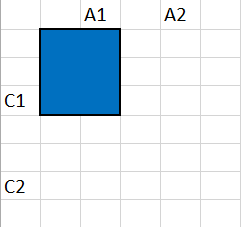
\includegraphics[width=7cm]{Imagenes/Ej3b.png}
\caption{Sueldo con $c_1$ y $a_1$}
\end{figure}

\begin{figure}[H]
\centering
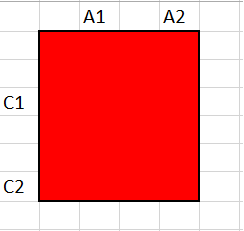
\includegraphics[width=7cm]{Imagenes/Ej3c.png}
\caption{Sueldo con $c_2$ y $a_2$}
\end{figure}

Las queries también pueden verse como suma de elementos de un rectángulo de la matriz. La query para los cargos y antigüedades del ejemplo anterior, se podría ver como la suma de los elementos del rectángulo de bordes ($c_1+1,a_1+1$), ($c_1+1,a_2$), ($c_2,a_1+1$) y ($c_2,a_2$).

\begin{figure}[H]
\centering
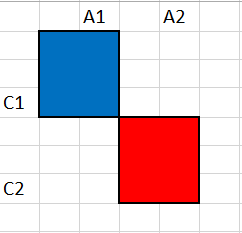
\includegraphics[width=7cm]{Imagenes/Ej3a.png}
\caption{Query con $c_1$, $c_2$, $a_1$ y $a_2$}
\end{figure}

En la figura puede verse en azul el sueldo con cargo $c_1$ y antigüedad $a_1$. En Rojo puede verse la parte que corresponde al sueldo con cargo $c_2$ y antigüedad $a_2$ pero que no puede obtenerse teniendo cargo $c_1$ o antigüedad $a_1$, que es lo que pide la query. Por lo tanto, la suma de los elementos del rectángulo rojo es la respuesta a la query.

Se decidió resolver el problema utilizando una tabla aditiva bidimensional. Sea una tabla aditiva $T$, la idea detrás de la tabla es que en la posición $T_{i,j}$ se encuentra $\sum_{i=1}^{c} \sum_{j=1}^{a} M_{i,j}$ (notar que esto es equivalente a \texttt{sueldo}($c_1,a_1$). Para resolver una query utilizando la tabla, se deben sumar y restar cuatro rectángulos.

La operación a realizar es la siguiente: $T_{c_2,a_2} - T_{c_1,a_2} - T_{c_2,a_1} + T_{c_1,a_1}$. 

En $T_{c_2,a_2}$ se encuentra el sueldo al que se aspira. Sería el rectángulo rojo de la figura del sueldo de $c_2$, $a_2$. Al sumar ese rectángulo se están sumando elementos de más. Por lo tanto, se proceden a restar otros dos rectángulos. Estos son  $T_{c_1,a_2}$ y $T_{c_2,a_1}$ y se pueden observar en las siguientes imagenes.

\begin{figure}[H]
\centering
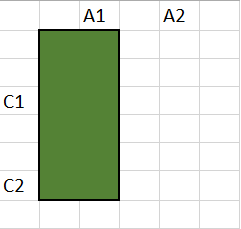
\includegraphics[width=7cm]{Imagenes/Ej3d.png}
\caption{Rectángulo correspondiente a $T_{c_2,a_1}$}
\end{figure}

\begin{figure}[H]
\centering
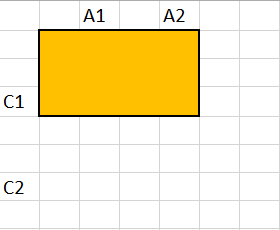
\includegraphics[width=7cm]{Imagenes/Ej3e.png}
\caption{Rectángulo correspondiente a $T_{c_1,a_2}$}
\end{figure}

Una vez restados estos dos rectángulos, se puede ver que el rectángulo correspondiente al sueldo con $c_1,a_1$ (el azul de la primer figura) se restó dos veces, una por cada uno de los dos rectángulos que se restó. Entonces se lo suma una vez. De esta forma lo que queda es el rectángulo rojo de la figura que muestra la resolución de la query. Entonces realizar esa cuenta en la tabla aditiva resuelve la query.

\subsection{Puntaje}
El peso otorgado a este ejercicio es:
